\documentclass{article}
\usepackage{graphicx} % Required for inserting images

\usepackage{amsmath}
\usepackage{amsfonts}
\usepackage{hyperref}
\usepackage{algorithm}
\usepackage[noend]{algpseudocode}

\usepackage{tikz}
\usepackage[margin=2.3cm]{geometry}

\usetikzlibrary{positioning}

\title{Computational Complexity -- Homework 2}
\author{Dario Halilovic\and
Antoni Jubés Monforte\and
Marcin Wojnarowski}

\date{31 November 2024}

\newcommand{\TQBF}[0]{\textsc{TQBF}}
\newcommand{\game}[0]{\textsc{3-ColourGame}}
\newcommand{\variantgame}[0]{\textsc{3-FixedColourGame}}
\newcommand{\PSPACE}[0]{\mathsf{PSPACE}}
\renewcommand{\P}[0]{\mathsf{P}}
\newcommand{\NP}[0]{\mathsf{NP}}
\newcommand{\SAT}[0]{\textsc{SAT}}

\begin{document}

\maketitle

\section*{Problem 1}

To prove $\NP^\SAT = \Sigma_2\P$ we prove both inclusions separately.

\subsection{$\NP^\SAT \subseteq \Sigma_2\P$}

Let $L \in \NP^\SAT$. By definition, there is a poly-time TM $M$ equipped with oracle access to $\SAT$ such that
\[
	x \in L \iff \exists y \, M^\SAT(x, y) = 1
\]
We construct a poly-time TM $M'$ that behaves as $M$ but has no access to the $\SAT$ oracle, instead relying on SAT answers and certificates as inputs. Specifically, for the $i$-th query, let $a_i$ be the oracle answer, $c_i$ the certificate assignment (if the answer is positive), and $w_i$ an arbitrary assignment (if the answer is negative). On input $x, \langle y, a_1, c_1, \ldots, a_m, c_m \rangle, \langle w_1, \ldots, w_m \rangle$, $M'$ runs as $M^{\SAT}(x, y)$, and when $M^{\SAT}$ performs its $i$-query to the oracle, it instead reaches for $a_i$ to get the answer:
\begin{enumerate}
	\item If $a_i$ is positive, $M'$ verifies that $c_i$ is a correct satisfying assignment, and rejects if that is not the case.
	\item Otherwise, it checks that $w_i$ is not a satisfying assignment (and rejects if $w_i$ is a valid assignment).
\end{enumerate}
Every step of $M'$ is poly-time bounded, thus $M'$ runs in polynomial time. Moreover, one has that
\[
	M^{\SAT}(x, y) = 1 \iff \exists a_1 \exists c_1 \forall w_1 \ldots \exists a_m \exists c_m \forall w_m \, M'(x, \langle y, a_1, c_1, \ldots, a_m, c_m \rangle, \langle w_1, \ldots, w_m \rangle) = 1
\]
where we quantify universally over assignments for unsatisfiable formulas. The choice of $w_i$ is independent of any $a_j$ or $c_j$ with $j>i$, so we can rewrite it as:
\[
	M^{\SAT}(x, y) = 1 \iff \exists a_1 \exists c_1 \ldots \exists a_m \exists c_m \forall w_1 \ldots \forall w_m \, M'(x, \langle y, a_1, c_1, \ldots, a_m, c_m \rangle, \langle w_1, \ldots, w_m \rangle) = 1
\]
Therefore,
\begin{align}
	x \in L & \iff \exists y \, M^\SAT(x, y) = 1 \nonumber                                                                                                                                                                                                                    \\
	        & \iff \exists y \, \exists a_1 \exists c_1 \, \cdots \, \exists a_m \exists c_m \, \forall w_1 \ldots \forall w_m\, M'(x, \langle y, a_1, c_1, \cdots, a_m, c_m \rangle, \langle w_1, \ldots, w_m \rangle) = 1 \nonumber                                         \\
	        & \iff \exists \underbrace{\langle y, a_1, c_1, \cdots, a_m, c_m\rangle}_{v_1} \, \forall \underbrace{\langle w_1, \ldots, w_m \rangle}_{v_2} \, M'(x, \langle y, a_1, c_1, \cdots, a_m, c_m \rangle, \langle w_1, \ldots, w_m \rangle) = 1 \label{eq:sigma_form}
\end{align}
Note that every variable is poly-size bounded and $m = \mathrm{poly}(x, y)$ since $M^{\SAT}$ makes polynomially many queries, therefore both $v_1$ and $v_2$ are polynomial size variables. This means that \autoref{eq:sigma_form} is of the $\Sigma_2\P$ form, and thus $L \in \Sigma_2\P$.


\subsection{$\Sigma_2\P \subseteq \NP^\SAT$}

Let $L \in \Sigma_2\P$. Then there is a TM $M$ such that
\[
	x \in L \iff \exists y \forall z \, M(x, y, z) = 1
\]
where $M$ runs in $\mathrm{poly}(x)$ time. Given $x$ and $y$, $\forall z \, M(x, y, z) = 1$ is a $\Pi_1\mathsf P = \mathsf{coNP}$ problem. But we know that $\mathsf{coNP} \subseteq \P^{\SAT}$. Let $M'$ be a poly-time TM with the $\SAT$ oracle that solves $\forall z \, M(x, y, z) = 1$.

We construct an NTM $N$ which chooses $y$ non-deterministically and runs $M'$. Then
\[
	x \in L \iff N(x) = 1
\]
Hence $L \in \NP^\SAT$ and thus $\NP^\SAT = \Sigma_2\P$.

\section*{Problem 2}

Define the set of oracles $\mathcal{A}$ as follows:
\[
	\mathcal{A} = \left\{ A \subseteq \{0, 1\}^*\,:\, \forall n \in \mathbb{N}, \, |A \cap \{0, 1\}^n| \in \{0, 2^{n-1}\} \right\}
\]
Given an oracle $A \in \mathcal{A}$, we define the language $L_A$:
\[
	L_A = \left\{ 1^n\,:\, |A \ \cap \ \{0,1\}^n|/2^n = \frac{1}{2} \right\}
\]

We have $L_A \in \mathsf{RP}^A$ for every $A$ in $\mathcal{A}$ since $L_A$ can be decided by an $\mathsf{RP}^A$ machine that, on input $1^n$, creates a random binary string $x \in \{0, 1\}^n$ and checks if $x \in A$. This machine accepts if $x \in A$ and rejects otherwise. As each string is equally likely to be chosen, the probability of acceptance is $1/2$ if $|A \cap \{0, 1\}^n| = 2^{n-1}$ (i.e. $1^n \in L_A$) and $0$ otherwise.
Thus, $\forall A \in \mathcal{A}$, $L_A \in \mathsf{RP}^A$.

Constructing $A$ such that $L_A \notin \mathsf{coRP}^A$ is more difficult. As done in an exercise, we will construct $A$ dynamically so that no $\mathsf{coRP}$ machine $M$ with oracle access to $A$ correctly decides $L_A$. In other words, we will find an oracle $A$ and language $L_A$ such that, for each $\mathsf{coRP}$ machine $M$ with access to the oracle $A$, there exists a string in the language $1^n \in L_A$ that outputs $M^A(1^n) = 0$ with non-zero probability, which violates the definition of a $\mathsf{coRP}$ machine.

Let $\mathcal{M}$ be the set of all $\mathsf{coRP}$ Turing machines that have an oracle access. This set is countable and hence there exists a sequence $(M_i)_{i \in \mathbb{N}}$ of deterministic Turing machines that contains all of $\mathcal{M}$. Furthermore, we impose that each $M \in \mathcal{M}$ appears infinitely many times\footnote{By the countable axiom of choice, a countable union of countable sets is countable, and therefore we can require each machine to appear infinitely many times in a countable enumeration.}.

We will construct $A$ dynamically, by specifying what elements of $\{0, 1\}^n$ it contains for increasingly larger values of $n$. To do so, it might be easier to think of $A$ as a function
\[
	A : \{0, 1\}^* \to \{0, 1, *\}
\]
where $A(x) = 0$ if $x \notin A$, $A(x) = 1$ if $x \in A$ and $A(x) = *$ if the membership is not yet fixed. We thus start with $A(x) := *$ for all $x \in \{0, 1\}^*$ and fix membership values on the fly.

For increasing values of $i = 0, 1, 2, \ldots$, we try to set $A$ in such a way that $M_i$ fails to decide $L_A$. At each step $i$, we run $M_i$ on input $1^i$ with oracle $A$, which will query $A$ only on the membership of some elements of length $i$. Whenever a membership query is made on input $x$, we set its undefined value $*$ to $A(x) := 0$. Even if $1^i \notin L_A$, some decider $M$ of $L_A$ could still accept $1^i$ with probability at most $1/2$. If $M_i$ accepts, we reset our membership to undefined for all length $i$, i.e., $A(x) := *$ for all $x$ of length $i$, and run the machine again. Almost surely, a decider $M$ for $L_A$ would eventually reject $1^i$ in finite time. We will assume $M_i$ will reject eventually. If it does not, $M_i$ already does not decide $L_A$, so we can fill the remaining $A(x)$ with $x$ of length $i$ to $0$ and go on to the next $i$.

If $M_i$ rejects $1^i$ with oracle $A$, we need to check how many values of $x$ of length $i$ were queried by $M_i$. Let $\Gamma = \{x_1, \ldots, x_p\}$ be the set of membership queries made to $A$ on this path. If $|\Gamma| > 2^{i-1}$, we set $A(x) = 0$ for all $x \in \{0, 1\}^i$ that are not in $\Gamma$ so that $1^i \notin L_A$, and we move on to the next $i$. Otherwise, if $|\Gamma| \leq 2^{i-1}$, we can choose $2^{i-1}$ strings of length $i$ that are not in $\Gamma$ and set $A(x) = 1$. Thus, on this instance which happens with non-zero probability, the $\mathsf{coRP}$ machine $M_i^A$ will be rejecting $1^i$ even though $1^i \in L_A$, ruling out $M_i^A$ as a decider for $L_A$.

Finally, since each $M \in \mathcal{M}$ appears infinitely many times in the sequence, at some point it must hold that $|\Gamma| = n^{O(1)} \leq 2^{n-1}$, causing at least one input to be wrongly decided by $M_i$.

Since there is no $\mathsf{coRP}$ machine that can decide $L_A$ with oracle $A$, we have that $L_A \notin \mathsf{coRP}^A$.

In conclusion, we have shown that for every $A \in \mathcal{A}$, $L_A \in \mathsf{RP}^A$; and that there exists an $A$ such that $L_A \notin \mathsf{coRP}^A$, which implies that $\mathsf{RP}^A \neq \mathsf{coRP}^A$ for some $A$.

\section*{Problem 3}

Define the following variant of the problem:
\begin{align*}
	\variantgame = \{\langle G, c \rangle \,:\, & G \textrm{ is a graph such that Alice has a winning}                          \\
	                                            & \textrm{strategy where every allowed 3-coloring } \hat{c} : V \to \{1, 2, 3\} \\ & \textrm{satisfies } \forall x \in \textrm{dom}(c), \hat{c}(x) = c(x) \}
\end{align*}
We argue that $\game \in \PSPACE$ by showing that we can solve $\variantgame$ recursively while re-using a polynomial amount of memory. Indeed, it is enough to solve $\variantgame$ since
\[
	\langle G \rangle \in \game \iff \langle G, \emptyset \rangle \in \variantgame
\]

Let $k(c) = \min(V \setminus \textrm{dom}(c))$ denote the minimal vertex $v \in V$ not in the domain of $c$. Notice that if $\textrm{dom}(c) \neq V$, one has
\begin{align*}
	\langle G, c \rangle \in \variantgame \iff \exists c_0\, \left\langle G, c \cup \{(k(c), c_0)\} \right\rangle \not\in \variantgame
\end{align*}
This gives us a recursive procedure to solve $\game$ as follows:

\begin{algorithm}
	\caption{Poly-space algorithm for $\game$}
	\label{alg:algorithm-label}
	\begin{algorithmic}[1]
		\Procedure{HasWinningStrategy}{$G, c$}
		\If{$\textrm{dom}(c) = V$ and $c$ is a 3-coloring of $G$}
		\State \Return {true}
		\EndIf
		\State $v \gets k(c)$
		\For{$c_0 \in \{1, 2, 3\}$}
		\If {$v$ can be colored by $c_0$ and \textsc{HasWinningStrategy}($G$, $c \cup \{(v, c_0)\}$) = false}
		\State \Return{true}
		\EndIf
		\EndFor

		\State \Return{false}
		\EndProcedure

		\vspace{1em}

		\Procedure{Solve3ColourGame}{$G$}
		\State \Return{\textsc{HasWinningStrategy}($G, \emptyset$)}
		\EndProcedure
	\end{algorithmic}
\end{algorithm}

The above algorithm needs $O(n^2)$ space to store $G$ and $c$, as well as
\[
	s(n) = s(n-1) + O(\log(n)) \leq O(n \log(n))
\]
space from the recursion, hence showing that $\game \in \PSPACE$.

To show that $\game$ is $\PSPACE$-complete, we reduce in polynomial-time from $\TQBF$. Without loss of generality, we may assume that the $\TQBF$ instance $I$ is of the form
\[
	\exists x_1 \forall x_2 \ldots \forall x_{n-1} \exists x_n \, \varphi(x_1, \ldots, x_n)
\]
where $\varphi$ is a CNF formula.

We construct a graph $G$ such that $\langle G \rangle \in \game$ if and only if $I \in \TQBF$. Our graph consists of four parts:
\begin{enumerate}
	\item First, a triangle composed of 3 vertices: $T$ (True), $F$ (False) and $B$ (Base). These 3 vertices are used to force a 3-coloring to pick a color for true and false assignments of a variable.

	\item Second, we create two vertices $x_i$ and $\overline{x_i}$ for every quantified variable $x_i$, connect them to each other, and connect them to vertex $B$.

	\item Third, we follow the encoding of CNF clauses used in the reduction from $\SAT$ to the decision version of 3-colorability. For each clause of the form $v_1 \lor v_2 \lor v_3 \lor \ldots \lor v_k = (((v_1 \lor v_2) \lor v_3) \lor \ldots ) \lor v_k$, we connect them by stacking OR-gadgets as follows:
	      \begin{figure}[H]
		      \centering
		      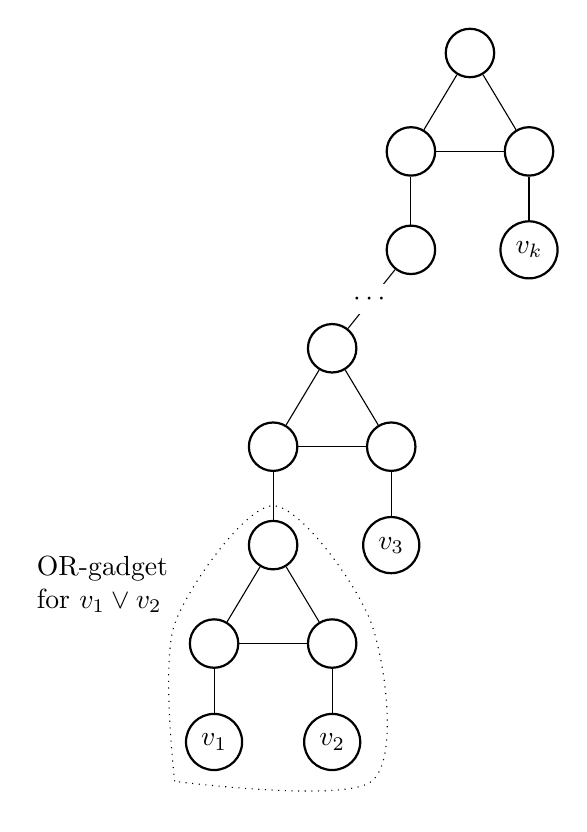
\begin{tikzpicture}
			      \begin{scope}[every node/.style={circle,thick,draw,minimum size = 1.75em}]
				      % First gadget
				      \node (v1) at (0,0) {$v_1$};
				      \node (v2) at (1.5,0) {$v_2$};
				      \node (above_v1) at (0,1.25) {};
				      \node (above_v2) at (1.5,1.25) {};
				      \node (middle_v1_v2) at (0.75, 2.5) {};

				      \draw (v1) -- (above_v1);
				      \draw (v2) -- (above_v2);
				      \draw (above_v1) -- (above_v2);
				      \draw (above_v1) -- (middle_v1_v2);
				      \draw (above_v2) -- (middle_v1_v2);

				      % Second gadget
				      \node (above_middle_v1_v2) at (0.75, 3.75) {};
				      \node (v3) at (2.25, 2.5) {$v_3$};
				      \node (above_v3) at (2.25, 3.75) {};
				      \node (middle_v1_v2_v3) at (1.5, 5) {};

				      \draw (middle_v1_v2) -- (above_middle_v1_v2);
				      \draw (v3) -- (above_v3);
				      \draw (above_v3) -- (above_middle_v1_v2);
				      \draw (above_v3) -- (middle_v1_v2_v3);
				      \draw (above_middle_v1_v2) -- (middle_v1_v2_v3);

				      % Third gadget
				      \node (stack) at (2.5, 6.25) {};
				      \node (above_stack) at (2.5, 7.5) {};
				      \node (vk) at (4, 6.25) {$v_k$};
				      \node (above_vk) at (4, 7.5) {};
				      \node (root) at (3.25, 8.75) {};

				      \draw (stack) -- (above_stack);
				      \draw (vk) -- (above_vk);
				      \draw (above_stack) -- (above_vk);
				      \draw (above_stack) -- (root);
				      \draw (above_vk) -- (root);
			      \end{scope}


			      \draw (middle_v1_v2_v3) -- (stack) node[midway,fill=white] {$\cdots$};

			      % Selected region
			      \draw[dotted] plot [smooth] coordinates {
					      (-0.5, -0.5)
					      (-0.5, 1.5)
					      (0.75, 3)
					      (2, 1.5)
					      (2, -0.5)
					      (-0.5, -0.5)
				      };
			      \node[text width=2cm] at (-1.25, 2) {OR-gadget for $v_1 \lor v_2$};
		      \end{tikzpicture}
		      \caption{Encoding of clause $v_1 \lor \ldots \lor v_k$}
		      \label{fig:clause-encoding}
	      \end{figure}

	      The top of the stack is then connected to the $B$ and $F$ vertices (so that any 3-coloring must color it with the same color as $T$).

	\item Fourth, we create a bunch of isolated "dummy" nodes, which will be used to let Alice effectively play multiple consecutive times by having Bob fill the color to these nodes.
\end{enumerate}

An example of the graph generated by the reduction is given in Figure~\ref{fig:full-example}.

\begin{figure}[H]
	\centering
	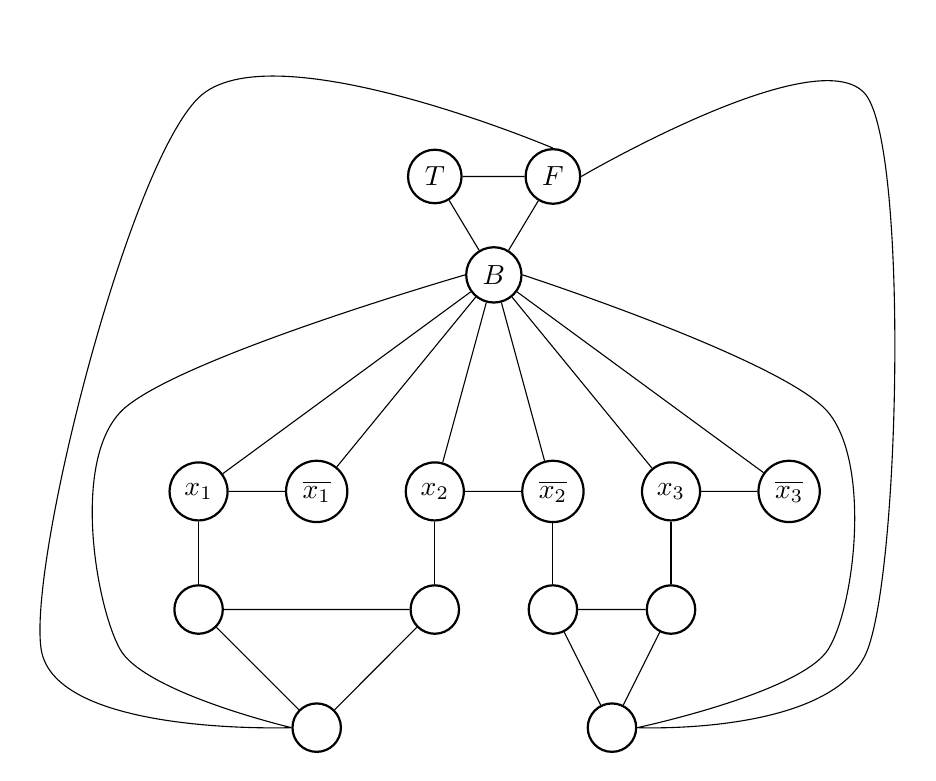
\begin{tikzpicture}
		\begin{scope}[every node/.style={circle,thick,draw,minimum size = 1.75em}]
			% First component
			\node (T) at (0,2) {$T$};
			\node (F) at (1.5,2) {$F$};
			\node (B) at (0.75, 0.75) {$B$};

			\draw (T) -- (F) -- (B) -- (T);

			% Variables
			\node (x1)     at (-3, -2) {$x_1$};
			\node (x1_neg) at (-1.5, -2) {$\overline{x_1}$};
			\draw (x1) -- (x1_neg) -- (B) -- (x1);

			\node (x2)     at (0, -2) {$x_2$};
			\node (x2_neg) at (1.5, -2) {$\overline{x_2}$};
			\draw (x2) -- (x2_neg) -- (B) -- (x2);

			\node (x3)     at (3, -2) {$x_3$};
			\node (x3_neg) at (4.5, -2) {$\overline{x_3}$};
			\draw (x3) -- (x3_neg) -- (B) -- (x3);

			% Gadgets
			\node (below_x1) at (-3, -3.5) {};
			\node (below_x2) at (0, -3.5) {};
			\node (middle_x1_x2) at (-1.5, -5) {};
			\draw (x1) -- (below_x1);
			\draw (x2) -- (below_x2);
			\draw (below_x1) -- (below_x2) -- (middle_x1_x2) -- (below_x1);

			\node (below_x2_neg) at (1.5, -3.5) {};
			\node (below_x3) at (3, -3.5) {};
			\node (middle_x2_neg_x3) at (2.25, -5) {};
			\draw (x2_neg) -- (below_x2_neg);
			\draw (x3) -- (below_x3);
			\draw (below_x2_neg) -- (below_x3) -- (middle_x2_neg_x3) -- (below_x2_neg);

			% Bent arrows for gadgets rule to B and F
			\draw plot [smooth] coordinates {
					(middle_x1_x2.west)
					(-4, -4)
					(-4, -1)
					(B.west)
				};
			\draw plot [smooth] coordinates {
					(middle_x1_x2.west)
					(-5, -4)
					(-3, 3)
					(F.north)
				};

			\draw plot [smooth] coordinates {
					(middle_x2_neg_x3.east)
					(5, -4)
					(5, -1)
					(B.east)
				};
			\draw plot [smooth] coordinates {
					(middle_x2_neg_x3.east)
					(5.5, -4)
					(5.5, 3)
					(F.east)
				};

		\end{scope}
	\end{tikzpicture}
	\caption{Graph (excluding dummy vertices) generated for the formula $\exists x_1 \forall x_2 \exists x_3 \, (x_1 \lor x_2) \land (\neg x_2 \lor x_3)$. A winning strategy for Alice would be to color $x_1$ and $x_3$ the same color as $T$, which make the OR-gadgets true irrespective of the color Bob chooses for $x_2$ ($T$ or $F$).}
	\label{fig:full-example}
\end{figure}

We now describe the order of processing Alice and Bob follow:
\begin{enumerate}
	\item First, Alice picks the colors for the $T$, $F$ and $B$ vertices, while Bob picks the colors for three different dummy nodes.
	\item Then, Alice and Bob successively pick a color for $x_i$, for $i = 1, \ldots, n$ (Alice starts by coloring $x_1$, then Bob picks $x_2$, and so on). Notice that since $x_i$ is connected to $B$, the chosen color is either that of vertex $T$ or $F$.
	\item Now, Alice picks the colors for $\overline{x_i}$ while Bob picks colors for dummy nodes. Since $\overline{x_i}$ is connected to $x_i$ and $B$, there is only one possibility for coloring $\overline{x_i}$.
	\item Finally, Alice plays alone on the rest of the graph, while Bob keeps coloring more dummy vertices.
\end{enumerate}
The reduction can be done in polynomial time, since the size of the graph is polynomial in the size of the formula and the number of variables.

Notice that Alice and Bob have picked an assignment of variables in phase 2, and the assignment makes the CNF true if and only if the remainder of the graph is 3-colorable. Therefore, Alice has a winning strategy if and only if, for every variable assignment that Bob makes, Alice can choose her variables accordingly to make the graph 3-colorable. Notice that since Alice plays alone at the end, the graph is 3-colorable if and only if Alice has a winning coloring.

This shows that Alice has a winning strategy if and only if $I \in \TQBF$, hence $\game$ is $\PSPACE$-complete.
\end{document}
